%
% Documento: Referencial Teórico
%

\chapter{Mobilidade Urbana em Cidades Inteligentes}\label{chap:Mobilidade Urbana em Cidades Inteligentes} %referencial teórico  

\begin{comment}
\mnote{Patrícia: Esse capítulo ainda tá um pouco confuso. As seções e subseções tem que conversar. Ainda parece um monte de coisa costurada. A ideia é começar a falar de Cidades Inteligentes e quando falar disso pega o que falamos naquela artigo, sobre a infraestrutura necessária e aí sim vc pode falar de computação e nuvem e PaaS, IaaS e SaaS. 
Na continuação sobre cidades inteligentes vc vai falar mais detalhadamente sobre mobilidade inteligente que é uma das dimensões que aquele autor propõe. Da uma olhada naquele artigo que a ideia eh aquela.
Quando vc falar de mobilidade vc insere o conceito de MaaS e somente depois de tudo isso vc falar sobre campus inteligente. 

Acho que nao cabe aqui ainda falar sobre carona solidária pq seu projeto mudou um pouco o foco devido todos os problemas. Vc vai falar de carona solidária somente na outra seção, quando for apresentar as soluções de mobilidade que foram encontradas, fará o comparativo e chegará na carona solidária.}

\end{comment}





%A imagem abaixo descreve bem as responsabilidades de cada camada da cloud:

\begin{comment}

\begin{figure}[!hbtp]
\centering
\caption{Camadas de Nuvem e suas responsabiidades.}
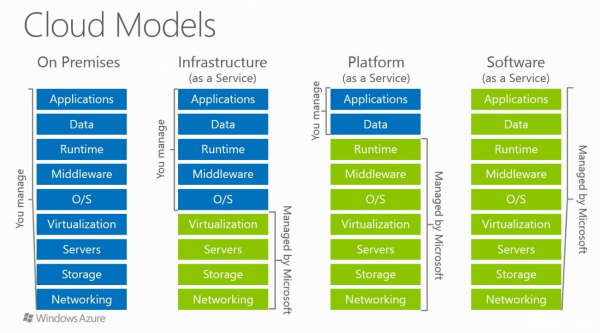
\includegraphics[width=8cm]{./04-figuras/azure-cloud.png}
\label{cloud-computing}
\fonte{https://www.lambda3.com.br/2017/08/iaas-paas-e-saas-qual-a-diferenca/}
\end{figure}
	conteúdo...
\end{comment}


\section{Cidades Inteligentes}

Cidades Digitais, CI, são cidades que utilizam um ambiente inovador caracterizado pela utilização de TIC. Segundo \citeonline{yin} os termos se referem a ação de utilizar a tecnologia em favor da melhoria da qualidade de vida, do gerenciamento de recursos e da infraestrutura das cidades.

Estas cidades sempre buscam otimizar recursos para melhor atender as necessidades dos cidadãos, interconectando informações, gerenciando operações sempre envolvendo uma infraestrutura tecnológica, sistemas inovadores e colaboração digital. \cite{washburn2010helping}.

% isso vale para mobilidade, para o setor imobiliário, saúde e entre outros serviços que de alguma forma podem ser otimizados usando TIC’s \cite{washburn2010helping}.

Já \citeonline{giffinger} acrescentam características para serem considerados antes de desenvolver uma CI. Para os autores, deve ser avaliado um todo, como consciência, flexibilidade, transformabilidade, individualidade, e comportamento estratégico da cidade e de seus cidadãos, e destaca que todos precisam ter conhecimento da posição da cidade e o que precisa ser feito para alcançar o status de CI. 

Segundo \citeonline{neirotti}, TIC não definem uma CI, são apenas uma das soluções utilizadas. O autor ainda explica que as cidades mais equipadas não implicam necessariamente nas melhores CI e o número de iniciativas não indicam performance, apenas demonstra o número de esforços para melhorar a vida dos cidadãos. 


\begin{comment}

De acordo com \citeonline{dameri}: 
\begin{citacao}
“Uma Cidade Inteligente é uma área geográfica bem definida, na qual altas tecnologias, como TIC, logística, produção de energia, etc., cooperam para criar benefícios para os cidadãos em termos de bem-estar, inclusão e participação, qualidade ambiental, desenvolvimento inteligente; é governado por um conjunto bem definido de assuntos, capaz de declarar as regras e políticas para o governo e o desenvolvimento da cidade”. (tradução nossa)."
%\footnote{Texto original: "A smart city is a well-defined geographical area, in which high technologies such as ICT, logistic, energy production, and so on, cooperate to create benefits for citizens in terms of well-being, inclusion and participation, environmental quality, intelligent development ; it is governed by a well-defined pool of subjects, able to state the rules and policy for the city government and development."}
\end{citacao}
\end{comment} 

CI em estudos de \citeonline{giffinger}, citado  por \citeonline{kon}, apresenta uma forma de como as cidades ditas inteligentes podem ser mensuradas e avaliadas, o mesmo cita 6 dimensões que possuem suas características próprias. Na Tabela \ref{tab:tabela1} veremos quais são:

% Please add the following required packages to your document preamble:
% \usepackage[table,xcdraw]{xcolor}
% If you use beamer only pass "xcolor=table" option, i.e. \documentclass[xcolor=table]{beamer}

\begin{table}[h]
\centering
\caption{Aspectos de Cidades Inteligentes}
\label{tab:tabela1}
\vspace{0.0cm}
\begin{tabular}{cp{10cm}}
\hline
 & Definição \\
\hline
\vspace{0.05cm}
Economia Inteligente & 
É a competitividade econômica, empreendedorismo, produtividade, leis que ajudem a inovar e incentivar a criação de novas soluções tecnológicas. \\
\hline
\vspace{0.05cm}
População Inteligente & 
Mede a qualidade da educação da população, seus postos de trabalho e renda, além de avaliar a interação social, os incentivos a programas de educação e incentivos a produção científica e tecnológica. \\
\hline
\vspace{0.05cm}
Governança Inteligente & Avalia o quão transparente e participativo é o governo por meio de seus portais, como são feitas as tomadas de decisões e serviços públicos e sociais.\\
\hline
\vspace{0.05cm}
Mobilidade Inteligente & Trata-se das questões de acessibilidade e mobilidade local onde se leva em consideração os congestionamentos, os transportes utilizados, o uso de combustível fóssil e as soluções tecnológicas que são utilizadas para melhorar o transporte da população.
% sempre priorizando os que menos prejudicam o meio ambiente e o fluxo urbano das cidades.
 \\
\hline
\vspace{0.05cm}
Ambiente Inteligente &
É avaliado quais soluções as cidades possuem para degradar menos o meio ambiente e quais recursos são reaproveitados, como água, energia, lixo.
% energia renovável, lixo reciclado e etc. 
\\
\hline
Vida Inteligente &
A qualidade de vida voltada para a segurança da cidade, da saúde das pessoas, o lazer, qualidade na moradia, serviços culturais.
%Este projeto tem como foco trabalhar apenas na mobilidade inteligente, que por meio de soluções tecnológicas tem melhorado bastante o fluxo nas ruas e estradas brasileiras.

\end{tabular}
\end{table}


\begin{comment}
	Contudo, CI não tem uma definição formal amplamente aceita, embora haja muitos conceitos sobre o tema, Cidade Digital é o que mais se destaca. Alguns autores abordam a diferença entre cidades inteligentes e cidades digitais.
	
	%%Sintetizar este paragrafo, muito grande
	%Segundo  \citeonline{yin}, 
	Cidades digitais se refere a digitalização de uma cidade, envolvendo informações, acesso ao dados e visualizações por parte da população, a cidade digital está mais ligada na forma em que a cidade utiliza e se moderniza com a combinação de comunicação e infraestrutura computacional para fornecer as informações públicas, já cidades inteligentes é uma definição que pode ser considerada como a junção do entendimento de cidade digital e sociedade do conhecimento, onde as pessoas envolvidas são responsáveis pelo aprimoramento do local criando zonas de colaboração digital \cite{yin}.
	%“o objetivo de uma cidade inteligente é transformar a vida e o trabalho dentro de uma região de maneira significativa e fundamental, não incremental” \cite{yin} (tradução nossa).
\end{comment}


Quando se fala a respeito do gerenciamento dos projetos de CI, \citeonline{chourabi} indicam que uma característica comum das iniciativas são que a maioria das cidades inteligentes são gerenciadas e organizadas por governos e utilizam o uso massivo de TIC. 

Uma iniciativa realizada no Brasil, até mencionada por \citeonline{namepardo}, é a da cidade de Porto Alegre, reconhecida nacionalmente e internacionalmente, a cidade tem tomado medidas usando tecnologia para o auxílio desde 2006 quando decidiu investir pesado na implementação de uma rede de fibra ótica para os serviços do governo , garantindo mais de 99.8 \% de disponibilidade \cite{weiss}.

 São Paulo se destaca também como o maior centro de pesquisa sobre o tema com muitas publicações e diversos trabalhos relacionados às áreas envolvidas, tendo a USP entre os destaques no número de publicações \cite{lazzaretti}. 


E para alcançarmos um nível de CI, algumas coisas precisam ser pensadas antes. Soluções que auxiliem questões como segurança, saúde, educação, ou mesmo lazer são fundamentais. Ações desde a construção de áreas verdes, de centros de cultura e monitoramento da cidade utilizando câmeras e mapeamento de zonas pouco seguras são essenciais. 

No entanto, a população não irá usufruir de nenhuma das soluções desenvolvidas para quaisquer das dimensões apontadas se não acontecer uma inclusão tecnológica massiva com programas de incentivo à educação científica e tecnológica. Caso contrário, parte da população será excluída e segregada da cidade \cite{patricia}.

Além disso, para construir uma CI fatores importantes como inclusão digital e infraestrutura tecnológica precisam ser discutidos. Para que estás soluções funcionem de maneira efetiva é necessário que elas sejam desenvolvidas considerando um sistema de computação que tenha uma arquitetura heterogênea e distribuída. As arquiteturas mais utilizadas atualmente são as em nuvem, devido sua capacidade de suportar grande demanda e a escalabilidade \cite{patricia}. 

\begin{comment}
	A arquitetura se dá primeiramente através de dispositivos de borda que são responsáveis por coletar dados dos dispositivos de internet da coisas espalhados pelo ambiente, a característica desses dispositivos é de serem de baixo processamento e capacidade. Após o processo de coleta, os dispositivos de borda enviam os dados para a nuvem para serem processados e armazenados. A rede tem características homogêneas com extrema importância de serem altamente disponíveis e capazes de oferecer acesso de milhares de pessoas por meio de seus dispositivos. Mais uma vantagem da computação em nuvem é se tratando de valores, segundo \cite{patricia}, a contratação de serviços em nuvem diminui os altos gastos em infraestrutura, a contratação conforme as necessidades das aplicações trazem uma grande vantagem, economia que não cria problema para os usuários, os serviços de nuvem oferecidos devolvem o resultado esperado.
\end{comment}

\subsection{Computação em Nuvem}
%encaixar a computação em nuvem no texto de cidades inteligentes, falar sobre sua importância para a construção de uma cidade inteligente e mencionar o artigo feito por nós
A Computação em Nuvem (\textit{Cloud Computing}) vem causando muitas transformações digitais e já tem um lugar de destaque nas CI. Embora atualmente seja algo bastante usual, esse é um assunto grande e complexo que possui vários subtemas, como os modelos de nuvem.

Dentro da Computação em nuvem é comum encontrarmos três modelos de disponibilização de serviços: 

Infraestrutura como serviço, oferece acesso baseado na web para armazenamento e poder de computação. O consumidor não precisa gerenciar ou controlar a subjacente infraestrutura em nuvem, mas tem controle sobre os sistemas operacionais, armazenamento, e aplicativos implantados.

Plataforma como serviço, onde os usuários hospedam um
ambiente para suas aplicações. Os usuários controlam os aplicativos, mas não controlam o sistema operacional, hardware ou infraestrutura de rede que são usados.

Software como serviço, é onde o consumidor usa um aplicativo, mas não controla o funcionamento do sistema, hardware ou infraestrutura de rede. Nesta situação, o usuário orienta os aplicativos pela rede. 

\citeonline{infra-cloud} diz que os serviços oferecidos pela Computação em Nuvem são semelhantes ao serviço de energia elétrica, pagamos apenas o que consumimos. Por consequência, necessidades como as de investir em equipamentos e infraestruturas de TIC são reduzidos.
% permitindo que seus usuários se conectem globalmente sem precisar implementar infraestruturas locais.

%consideravelmente, permitindo que seus usuários se conectem e façam colaborações globalmente sem configurar
%infraestruturas, como servidores, e com uma alta escalabilidade e capacidade de acomodar inúmeros usuários. 

%que seus usuários se conectem globalmente sem precisarem configurar infraestruturas de TI locais.

Vale ressaltar que a capacidade de uma CI ser dinâmica e automática faz ela precisar de infraestruturas robustas e capazes de suprir as necessidades de estar todo tempo online, algo que a computação em nuvem consegue oferecer através de serviços altamente disponíveis, elásticos, flexíveis e robustos. \cite{kon-cloud}.


\section{Mobilidade Inteligente}
%\mnote{compartilhamento de carros}
%\mnote{compartilhamento de viagens}
%\mnote{transporte sob demanda}
%\mnote{Falar sobre as tecnologias que tornam possível a utilização de ferramentas de mobilidade inteligente; gps, smartphones, cloud}
%Com o passar dos anos, A mobilidade urbana está necessitando cada vez mais de atenção. 

%Com o aumento do número de pessoas e veículos surgem alguns problemas  como engarrafamentos cada vez maiores, dificuldade de locomoção de pedestres e ciclistas, poluição do ar. 

%No entanto, \citeonline{santana} diz que a Mobilidade Urbana vai além de trânsito lento e grandes congestionamentos, a mobilidade urbana carrega a importância da cidadania de um povo.

\citeonline{giffinger} afirma que mobilidade inteligente trata-se de acessibilidade nacional e internacional dando importância as tecnologias modernas advindas da TIC e sistemas de transporte sustentáveis. O uso de uma tecnologia moderna que dê suporte a mobilidade faz surgir sistemas “inteligentes”.

Além disso, otimizar a logística dentro de áreas urbanas, fornecer aos cidadãos um sistema dinâmico e multimodal, assegurar um transporte sustentável e ecológico e ainda considerar as condições de tráfego e energia melhoram o trânsito urbano e mobilidade dos habitantes \cite{neirotti}. %\cite{giffinger}.

Modais como ônibus, metrôs, carros e bicicletas são avaliados em relação a sua facilidade de mobilidade. Analisar o tamanho da malha viária, ciclovias, uso de transportes poluentes e não poluentes também são parâmetros considerados \cite{kon}. 

%Muitas iniciativas e soluções tecnológicas com objetivos de tratar essas "dores" \cite{cocchia} Como resultado, este livro dedica vários capítulos ao debate sobre como medir
%o impacto das iniciativas de cidades inteligentes na criação de valor público para as pessoas
%que vivem, trabalham, estudam e visitam uma cidade.

Atualmente é possível monitorar todo e qualquer tipo de transporte, o GPS é um dos dispositivos que nos auxiliam nisso. Na cidade de São Paulo, a Startup Scipopulis monitora em tempo real 14 mil ônibus obtendo dados da velocidade média das vias, informações sobre acidentes, número de ônibus transitando na mesma via. Todos essas informações são passadas para a companhia da transporte da cidade para possíveis melhorias na mobilidade da cidade de São Paulo \cite{kon}.

Dois projetos na cidade de Madri (Espanha) que utilizam o GPS dos celulares dos cidadãos são dignos de nota, um de monitoramento em tempo real da posição do transporte publico e outro estimando a lotação dos coletivos. Amsterdã também tem projetos voltados para o controle e monitoramento do trânsito, alguns projetos interessantes que são realizado na capital holandesa é o incentivo de carros elétricos, disponibilizando vários pontos de recarga pela cidade \cite{kon}.


%Diante do exposto, a Mobilidade Urbana

%Das várias iniciativas de cidades inteligentes, a mobilidade tem um lugar de destaque por apresentar várias soluções que já apresentam uma melhora no trajeto das pessoas em várias cidades utilizando TIC. 



% a exemplo disso, aplicativos como Uber, 99 circulam pelas cidades utilizando a mobilidade como um serviço.

%Aplicativos de carona como o BlaBlaCar  que a relação entre o motorista e o passageiro fica a critério do motorista em relação aos custos da viagem. Estas ferramentas já contribuem com a melhoria da mobilidade sem a necessidade de investimento público. 

%Uma mudança que estas aplicações apresentam é a de lugares ocupados dentro de um mesmo veículo. Segundo pesquisa realizada pela BlablaCar em 2018, a taxa de ocupação de pessoas usando o aplicativo por veículo no Brasil é de 3,8 incluindo o motorista, contra 1,9 pessoas por veículo sem o uso de do aplicativo, na mesma pesquisa, a empresa apresenta dados que as caronas solidárias ajudam na economia de CO² alegando que pessoas que  fazem o mesmo trajeto todo dia e possuem carros podem participar de um rodízio de caronas, por exemplo, nesta conta, teríamos todo dia 1 carro a menos nas ruas.

%Hoje em dia são algumas dessas soluções, aplicativos como BlaBlaCar, outros aplicativos de carona solidária mobilizado por universidades como o Caronaê da UFRJ\footnote{Disponível em: https://caronae.org/. Acesso em: 23 Jun. 2020.}, entre outras,  que movimentam o conceito de mobilidade urbana inteligente no país.

%1 - O que é?

%2 - A mobildade urbana e inteligente

%3 - A importancia da mobilidade inteligente

% serviços já existentes (uber, 99, falar um pouco de maas); mobilidade como serviço
% carona solidária

%Cocchia (2014) -a adoção de políticas de crescimento requer que as cidades
%passem a buscar projetos com o fornecimento de soluções para mobilidade urbana. As cidades
%inteligentes incialmente eram chamadas de cidades digitais por incorporar ao seu conceito
%apenas o uso de tecnologia da informação. Com a evolução passaram a incluir os conceitos de
%sustentabilidade aos seus projetos. A mobilidade urbana em cidades inteligentes faz surgir o
%5conceito da “mobilidade urbana inteligente”.

\section{Campus Inteligente}

Um campus inteligente é o reflexo de uma cidade em uma escala menor, nos campos temos relações sociais, relações administrativas, meio ambiente, serviços de coleta, mobilidade, alimentação, energia, entre outros.

Conforme \citeonline{zhang}, o comportamento de uma Campus Universitário Inteligente é semelhante ao de uma CI, porém, com um número de problemas menores, e de proporções menores, onde pode ocorrer roubos, acidentes de carro, circulação de pessoas em lugares proibidos ou outras situações não permitidas \cite{garay2018}.

Assim como cidades inteligentes, campus inteligente ou universidade inteligente não tem um conceito totalmente definido, \citeonline{alghamdi} explica que o campus inteligente surge da necessidade de oferecer serviços de alta qualidade reduzindo custos, e que isso não fica apenas nos aspectos acadêmicos, mas envolve aspectos sociais, meio ambiente, e financeiros da Universidade.

\begin{comment}
Na Figura \ref{alghamdi}, temos:
\begin{figure}[!hbtp]
\centering
\caption{Conceito de Campus Inteligente, seu impactos e suas aplicações.}
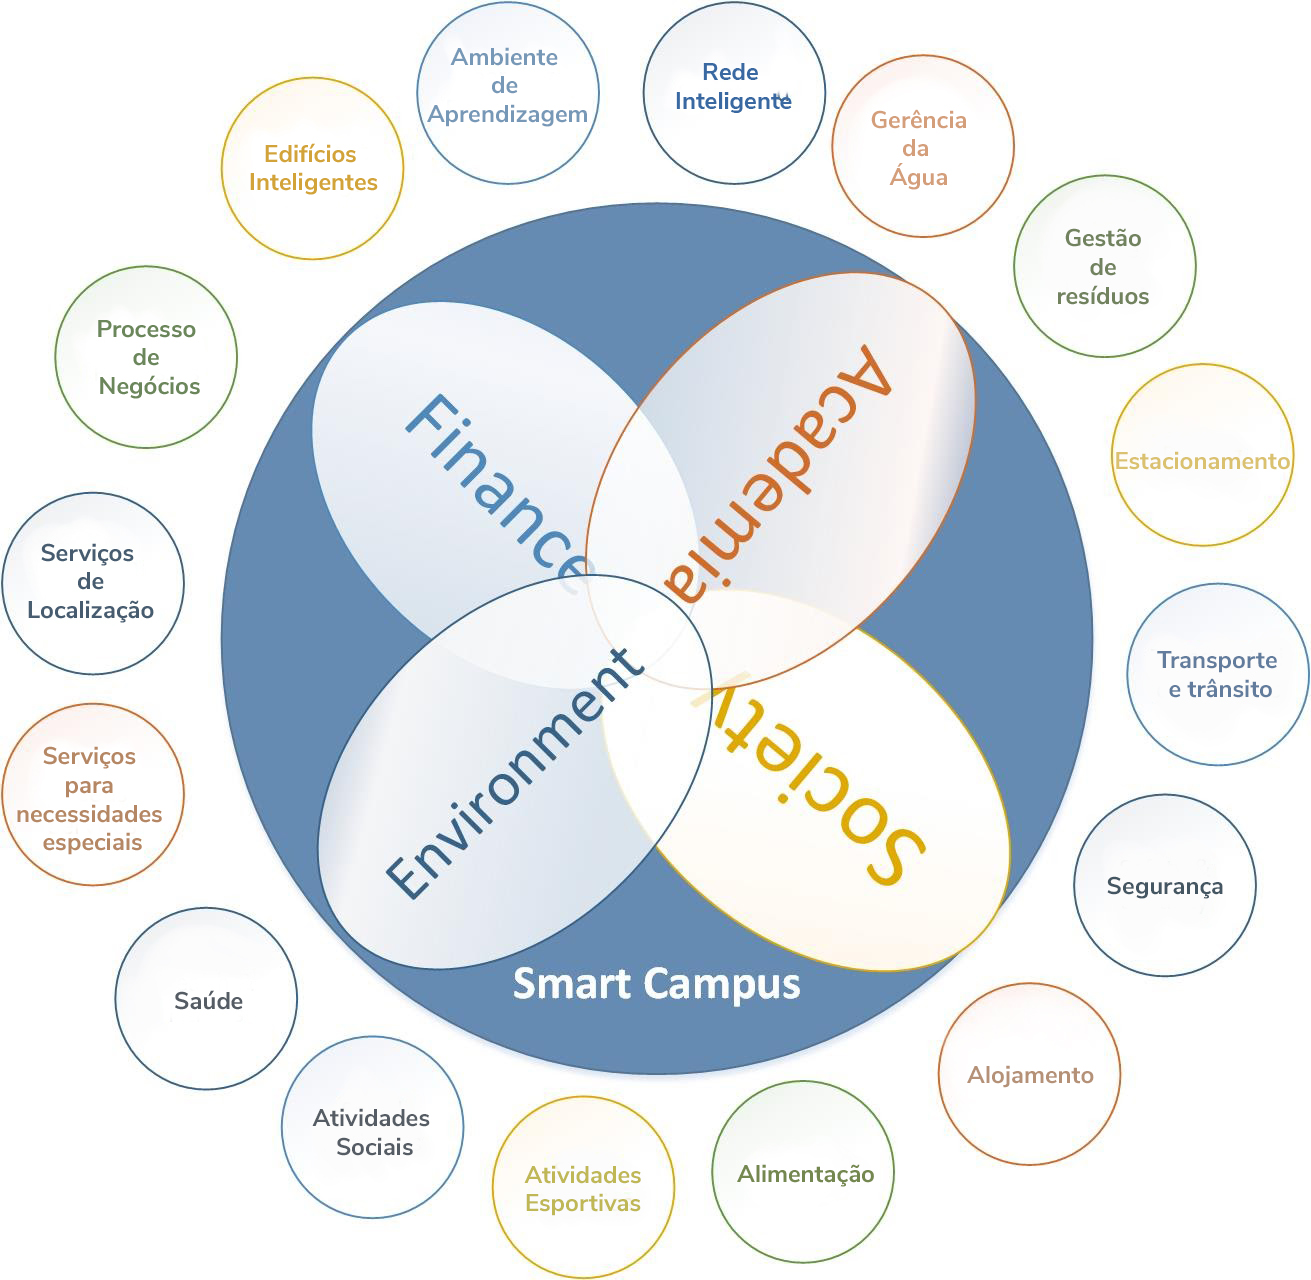
\includegraphics[width=8cm]{./04-figuras/alghamdi-edited.jpg}
\label{alghamdi}
\fonte{Adaptado de \citeonline{alghamdi}}
\end{figure}
\end{comment}




Além do conceitos e objetivos, o Campus Inteligente também tem problemas e dificuldades que o mercado impõe. \cite{alghamdi} cita 3 obstáculos: Técnico, Financeiro e Político. Semelhante as Cidades Inteligentes, deve-se considerar que ao estabelecer serviços tecnológicos a uma população, que seja de uma cidade, ou de uma universidade, conceitos de segurança, proteção e privacidade, interoperabilidade, padronização e configurações precisam estar bem encaixados para promover segurança ao uso por pessoas do Campus/Cidade, e reunir esses requisitos num ambiente tão heterogêneo, de comunicação intensiva é uma tarefa difícil \cite{alghamdi}. 

Do lado financeiro, conseguir dinheiro para levar adiante projetos que necessitam de investimentos algumas vezes elevados e experiências imaturas, ou até mesmo, sem experiência alguma com Campus Inteligente acaba dificultando iniciativas ao redor do mundo . Finalmente, os obstáculos políticos em um ambiente universitário
não são tão difíceis quanto as técnicas e financeiras devido ao
fato de que o presidente de uma universidade pode resolver a tomada de decisão processo em muitos casos; no entanto, a colaboração entre
diferentes faculdades e departamentos, reengenharia de negócios
processos e oposição de funcionários anti-tecnologia são potenciais
obstáculos que precisam ser resolvidos \cite{alghamdi}.

Por outro lado, as iniciativas tecnológicas abrem portas para recrutarmos pesquisadores, investigarmos mais sobre o tema e promover serviços e soluções inovadoras, segundo \cite{alghamdi}, a maioria dos trabalhos focados em Campus Inteligentes são sobre energia, meio ambiente e prédios inteligentes, e alguns serviços importantes, como transporte, alimentação, controle de tráfego ficam deixadas de lado.

\section{Mobilidade com Serviço - MaaS}

Mobilidade como um serviço (Mobility as a Service) é um termo utilizado para nomear uma nova tendência na mobilidade inteligente, onde empresas, organizações investem no transporte público oferecendo meios multimodais de locomoção  para a população. Algumas das características de plataformas MaaS é a facilidade de acesso, a ferramenta apresenta as opções que o usuário pode escolher para seu trajeto, facilidade no pagamento, sistema de reserva de viagens e informação em tempo real.

Sem uma definição exata, o MaaS é definido por alguns autores como a oferta de serviços de mobilidade centralizados em uma única plataforma digital, focando exclusivamente nas necessidades individuais dos usuários, sendo estes, táxis, transporte público coletivo, carros particulares, bicicletas, entre outros \cite{jittrapirom, kamargianni, mulley}.

Para não aprofundar, o objetivo da MaaS é incentivar o uso de transportes compartilhados e que seja possível o usuário planejar o seu trajeto em cima de várias opções multimodais, sejam elas, compartilhamento de carros, caronas, compartilhamentos de bicicletas, aluguel de carros, transporte público, entre outros meios de mobilidade \cite{jittrapirom}. 

\subsection{Soluções de Mobilidade}

%Carros híbridos, carros elétricos, patinetes elétricos, compartilhamento de carros. chips, gps,smartcards, protocolo its são responsável por isso ser possível

%\textbf{Como FUNCIONA, PERGUNTA A SER FEITA PARA CADA SOLUÇÃO DE MOBILIDADE INTELIGENTE}

A mobilidade urbana e o transporte são vitais para o funcionamento das cidades inteligentes. Mobilidade urbana significa acessibilidade local, nacional e internacional da CI, disponibilidade de infraestrutura de TIC, bem como sistema de transporte inovador e seguro.  O atual surgimento de soluções sistêmicas nos transportes é uma parte do movimento em direção à mobilidade sustentável. Permite não só o bom desenvolvimento de uma cidade, mas também ajuda a superar dificuldades notadamente visíveis em áreas urbanizadas e densamente inibidas, como engarrafamentos, emissões poluentes, congestionamento sonoro, separação de espaços habitacionais e outros \cite{opitek}.

Para \citeonline{dameri}, o envolvimento das TICs proporcionou inúmeras iniciativas para cidades inteligentes, como por exemplo monitorar a mobilidade urbana inteligente e outras tecnologias como redes inteligentes, veículos de combustível alternativo e assim por diante, o autor ainda afirma que cada tecnologia incentiva várias outras iniciativas e projetos que podem melhorar a qualidade de vida, a redução da poluição, a redução dos congestionamentos, entre outros.

A exemplo dessas tecnologias, foi através do GPS que muitas iniciativas foram postas em prática. A tecnologia  que disponibiliza a localização em tempo real foi responsável pelo surgimento de mapas digitais -- A ferramenta Google Maps é um exemplo claro disso -- que desencadeou uma série de soluções de mobilidade inteligentes. Soluções que fornecem a localização em tempo real de transportes coletivos, de veículos, pessoas, que possibilita planejar um itinerário, de saber onde outra pessoa se encontra e podendo verificar o melhor trajeto para chegar até ela, são uma das várias soluções existentes e possíveis de encontrar atualmente.

E para isso, vamos exemplificar algumas das categorias dessas opções de mobilidade existentes que nos  dividimos em 4 modalidades:
% Nome dos novos tópicos
\begin{itemize}
	\item Orientações de Mobilidade
	\item Transporte Individual Privado de Passageiros por Aplicativo
	\item Viagens Compartilhadas por Aplicativos
	\item Veículos Compartilhados
\end{itemize}

\section{Orientações de mobilidade}

Essa categoria agrupa plataformas que atuam no auxílio à orientação para os deslocamentos da cidade. Portanto, são usadas indistintamente por motoristas a serviço de outros ou pelos próprios indivíduos em deslocamento. Os exemplos mais conhecidos são o Google Maps e o Waze Mobile, ambos presentes em vários países. Como se baseiam no sinal de GPS, que tem
abrangência mundial, são frequentemente escalonáveis para corresponder a essa abrangência,
dependendo apenas do efetivo mapeamento de ruas. \cite{caronae}

%Dissertação de Luísa (texto sem mudanças)

\subsection{Waze}

A Waze foi fundada em 2008 em Israel, originalmente chamada de LinQmap, e em 2011 já
empregava 80 pessoas. Seu diferencial, se comparada aos sistemas de navegação por GPS tradicionais, vem do fato de se basear em uma comunidade de usuários, aproveitando-se da localização fornecida por cada usuário através de seus Smartphones. 
%para alimentar seu banco de dados.
% Foi a primeira plataforma a funcionar desta forma, antes mesmo da Google lançar essa funcionalidade em seu aplicativo de mapas. As informações enviadas pelos usuários possibilitam a atualização da plataforma em tempo real, gerando informações muito precisas sobre o fluxo de tráfego, por exemplo.

Daí inferimos outra categoria de classificação importante, do ponto de vista da mobilidade
urbana: aplicativos uni ou multimodais. O Waze, desse ponto de vista, por ser uni modal – e o modal em questão ser o carro particular –, pode melhorar as escolhas de trajetos dos motoristas, aliviando o tráfego e diminuindo o tempo de viagem.
% o Google Maps, ao permitir a visualização de diferentes tempos de deslocamento segundo cada modal (de carro, de ônibus, a pé, de bicicleta ou mesmo de avião, quando o trajeto permite), estimula a exploração dos diferentes modais (ainda que a combinação de modais para um mesmo trajeto seja ainda pouco explorada), o que pode acabar levando a escolhas mais sustentáveis, em especial para deslocamentos menores. 

%Dissertação de Luísa (texto sem mudanças)

\subsection{Cittamobi}
O Cittamobi é um aplicativo de transporte público disponível em plataformas iOS e Android com finalidade de fornecer mapeamento, cadastros, monitoramento, previsões e informações de ônibus, linha e rotas calculadas em tempo real. O aplicativo utiliza a localização atual do usuário e o local de destino para encontrar o ponto de ônibus, a linha e o tempo que cada veículo vai demorar até chegar. Na figura \ref{fig:cittamobi} vemos algumas telas do aplicativo Cittamobi.

\begin{figure}[!hbtp]
	\centering
	\caption{Telas do aplicativo de orientações de mobilidade Cittamobi}
	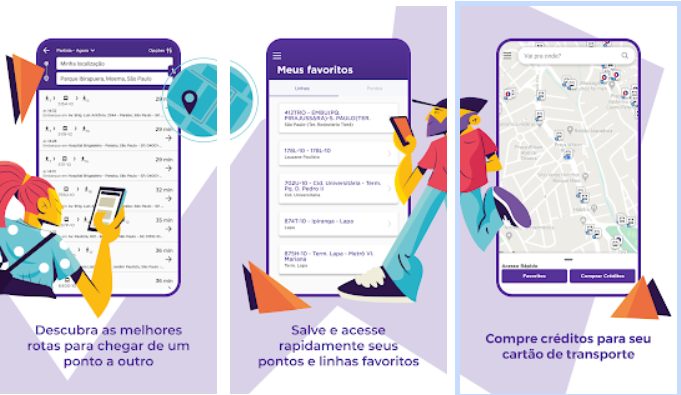
\includegraphics[width=0.4	\textwidth]{./04-figuras/cittamobi/cittamobi.png}
	\label{fig:cittamobi}
	\fonte{Loja de aplicativos do Android: PlayStore}
\end{figure}



%\subsection{Moovit}

\section{Transporte Individual Privado de Passageiros por Aplicativo}

A mobilidade vem mudando durante os anos, surgem novas maneiras e ferramentas para o uso da mobilidade, aplicativos como Uber, Cabify, BlaBlaCar, Yet Go, entraram no mercado e se tornaram ferramentas muito úteis, de grande uso, e ajudando tanto na mobilidade da população quanto no trânsito de muitas cidades, levando em consideração que pessoas que utilizam bastante deixam de ter a necessidade de possuir um carro para utilizar apenas esses serviços, baseado no conceito de consumo compartilhado que vimos anteriormente.

Esse novo conceito, essa nova abordagem de mobilidade é inserida nas cidades não apenas com as ferramentas citadas acima, mas outras iniciativas, como de universidades também tentam melhorar a mobilidade de seus determinados públicos através de aplicativos de carona solidária, pontos de parada de compartilhamento de corridas.

Inspiradas pelo crescente sucesso da Uber, surgiram startups visando de atuar de forma similar, mas voltados para o mercado de motoristas de táxi, algumas delas cresceram e se destacam por sua abrangência cada vez maior, como é o caso da Easy Taxi, empresa brasileira fundada em 2012 no Rio de Janeiro, presente em mais de 30 países e 420 cidades atualmente \cite{caronae}.
%texto não modificado

\subsection{Uber}
A história da Uber teve início quando seus fundadores, Garrett Camp e Travis Kalanick, em Paris, encontraram certa dificuldade para encontrar um táxi. Percebendo a demanda por transporte, os executivos resolveram criar uma plataforma que permitisse solicitar carros premium. A Uber foi fundada em 2009, na Califórnia, como um aplicativo para facilitar o acesso ao transporte.

A Uber chegou ao Brasil em 2014, com atuação no Rio de Janeiro. A segunda cidade a receber o aplicativo foi São Paulo, seguida por Belo Horizonte. Atualmente, mais de 100 cidades brasileiras contam com os serviços da empresa, realizados por 500 mil motoristas parceiros. 

%https://canaltech.com.br/empresa/uber/#:~:text=A%20hist%C3%B3ria%20da%20Uber%20teve,dificuldade%20para%20encontrar%20um%20t%C3%A1xi.&text=A%20Uber%20foi%20fundada%20em,facilitar%20o%20acesso%20ao%20transporte.

\begin{comment}
\subsection{99}
Fundada em 2012, a 99 é fruto da vontade de fazer diferente de três conhecidos geeks da internet brasileira: Ariel Lambrecht, Renato Freitas e Paulo Veras. Seis anos depois, fomos adquiridos pela DiDi, a maior plataforma de transporte por celular do mundo que atinge mais de 60\% da população mundial e cobre mais de mil cidades com um serviço de mobilidade cada dia melhor. Além do nosso trabalho constante pelo melhor serviço, perseguimos a missão de impactar positivamente a população, tornando o transporte mais barato, rápido e seguro para passageiros e o dia a dia mais rentável e tranquilo para motoristas através da tecnologia. E para que isso aconteça, damos poder de escolha para todos com as nossas categorias de serviço, que vão desde o 99Pop, com motoristas particulares em diversas cidades; até o 99Táxi, presente em todo o Brasil no modo tarifa cheia e desconto, que oferece a comodidade do táxi com valores até 30\% mais baixos; e o 99Top, um serviço premium com táxis de luxo. Assim, no brasil, conectamos 14 milhões de passageiros a 300 mil taxistas e motoristas e mudamos a vida de milhões de pessoas todos os dias, reinventando o seu jeito de ir e vir. 
%https://www.revelo.com.br/empresas/99taxis

\end{comment}

\subsection{Cabify}

Cabify é um dos grandes nomes no seguimento de aplicativos de viagem e deslocamento. A empresa é conhecida como uma multinacional de rede transporte, concorrente de outros serviços como, por exemplo, Uber e 99.

Em Cabify, a dinâmica é bem parecida com outros aplicativos de carona no mercado, seus usuários podem pedir por corridas para lugares determinados através de sua geolocalização.

No entanto, a plataforma conta com alguns diferenciais oferecendo o serviço de táxis e motoristas profissionais, além disso, é possível programar corridas de acordo com o dia e horário desejados, recurso que ainda foi pouco explorado por outros aplicativos. 

%https://canaltech.com.br/apps/cabify-o-que-e-como-funciona/%

\section{Viagens Compartilhadas por Aplicativos}
\subsection{BlaBlaCar}

O BlaBlaCar é um aplicativo de caronas bastante utilizado para corridas intermunicipais, o valor fica a critério do caroneiro em negociação com o motorista. O aplicativo surgiu em meados de 2003 devido a necessidade de Fred (Fundador da BlaBlaCar) de ir visitar sua família no interior da França sem carro e com as passagens de trem esgotadas, ele pediu que sua irmã fosse buscá-lo, durante o caminho, ele notou que muitos carros andavam com muitos lugares desocupados, então, ele viu nessa situação um começo de um novo modal (BlaBlaCar, 2020).

O aplicativo é diferente dos citados acima por ser aberto para todos, basta realizar o cadastro e já pode compartilhar suas caronas. Comparado a outros aplicativos voltados à remuneração como Uber e 99, o BlaBlaCar costuma ter viagens mais longas, intermunicipais por exemplo, à um preço bem mais acessível. %texto escrito por mim

\subsection{Bynd}

A empresa foi criada no final de 2014 em decorrência de uma experiência pessoal de seus dois sócios-fundadores, Gustavo Bertazzola Graciteli e Leonardo Fernandes Libório, que fizeram uma viagem pelas Américas por 13 meses em um carro compartilhado com outras três pessoas. Após esse período sabático, ambos decidiram abandonar suas carreiras no mercado financeiro e iniciar um novo negócio. A ideia de criar a Bynd surgiu em uma palestra para empreendedores. na qual um dos diretores da Tecnisa (empresa do mercado imobiliário brasileiro) apresentou problemas que careciam de soluções mais eficazes; entre elas, a dificuldade em disponibilizar vagas de estacionamento aos funcionários da empresa. Assim, a Bynd surgiu para melhorar a taxa de ocupação dos veículos, melhorando a eficiência dos deslocamentos realizados por meio de carons corporativas.

% texto da Tesé André

O suporte da tecnologia da informação e comunicação foi imprescindivel para a que a Bynd oferecesse seus serviços, entre eles: a disponibilização do aplicativo para dispositivos móveis e do \textit{website}; a implementação de salas de bate-papo para facilitar a comunicação direta entre os usuários; a realização de atendimentos virtuais; o desenvolvimento dos mecanismos de premiação e de incentivos; as consultas às caronas disponíveis em tempo real; o envio de notificações, entre outros. Embora cientes da possibilidade de extrair dados de dispositivos da Internet das Coisas e de \textit{big data}, esses recursos ainda não foram implementados; contudo, os fundadores ressaltam que a previsibilidade e a confiabilidade são requisitos essenciais para a operação de seu modelo de negócio, e ambos são suportados pelas TIC. 

%texto da tese André

\subsection{Vemcar}

Desenvolvido na Universidade Federal do Rio Grande do Norte, o aplicativo Vemcar começou a ser desenvolvido em uma disciplina oferecida no curso de Engenharia de Software, logo após, o protótipo passou para a equipe da Superintendência de Informática da Universidade Federal do Rio Grande do Norte (SINFO), lá foi realizado toda a validação da ideia, surgimento dos requisitos e foram aplicadas as regras do um processo de software. No Vemcar somentes pessoas ligadas à universidade( professores, alunos, técnicos) podem utilizar o aplicativo.

%texto escrito por mim

\begin{figure}[!hbtp]
	\centering
	\caption{Aplicativo de Carona Solidária Vemcar}
	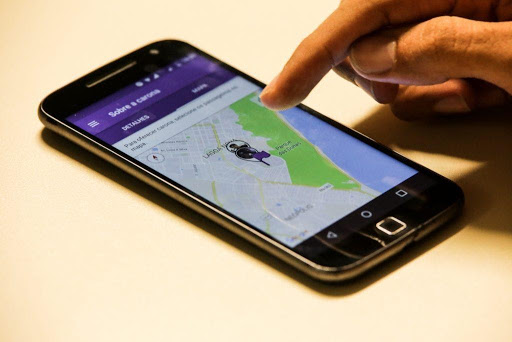
\includegraphics[width=0.5\textwidth]{./04-figuras/vemcar.jpg}
	\label{fig:tecnologia}
	\fonte{https://www.ufrn.br/imprensa/materias-especiais/2872/aplicativo-de-caronas-solidarias-da-ufrn-registra-mil-downloads-em-uma-semana}
\end{figure}


\subsection{Caronaê}

%mencionar trabalho da luísa e do artigo publicado sobre o aplcativo.

O Caronaê é um aplicativo de carona voltada para o ambiente universitário desenvolvido por alunos da Universidade Federal do Rio de Janeiro (UFRJ). O aplicativo está disponível para duas plataformas, Android e iOS. Em seu site oficial (CARONAÊ, 2020) diz que \textit{“O Caronaê é um sistema de código aberto, seguro e prático de caronas compartilhadas, criado com o objetivo de ser replicado em diferentes instituições e feito exclusivamente para a comunidade acadêmica das instituições integrantes da Rede Caronaê”}.

Dos pontos interessantes que o aplicativo oferece são, o uso exclusivo da comunidade acadêmica, a centralização das ofertas de carona, o aumento da taxa de ocupação dos veículos e pontos de carona para facilitar o encontro de caroneiro e carona. A Figura~\ref{fig:caronae} mostra a tela inicial do site do aplicativo de carona \textbf{Caronaê}.

\begin{figure}[!hbtp]
	\centering
	\caption{Aplicativo de Carona Solidária Caronaê}
	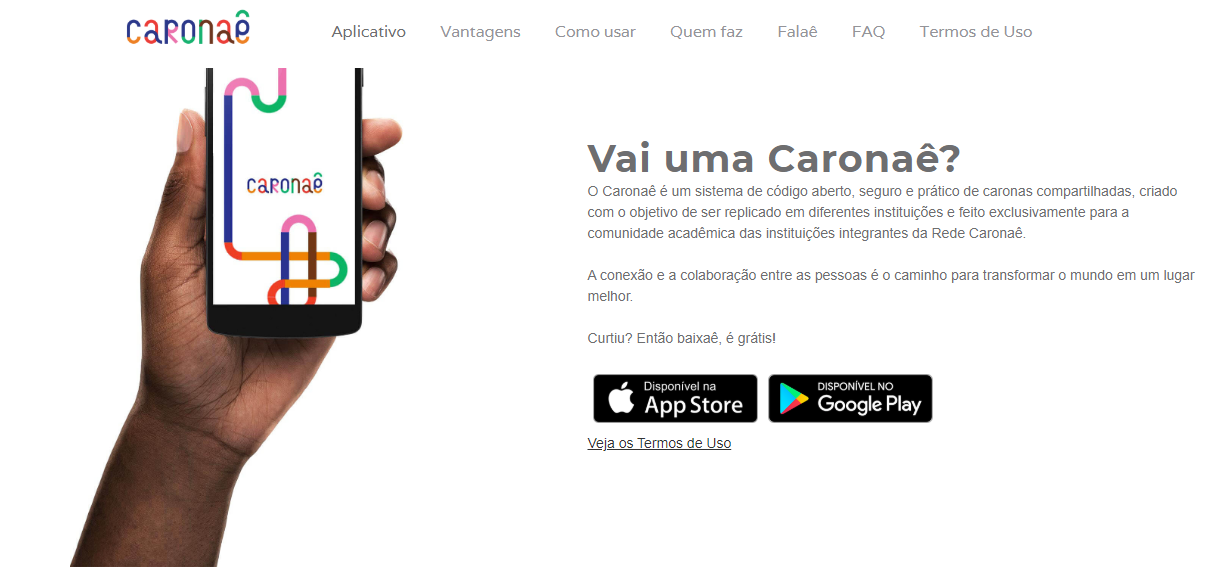
\includegraphics[width=0.8\textwidth]{./04-figuras/caronae.png}
	\label{fig:caronae}
	\fonte{https://caronae.org/index.html}
\end{figure}


%texto escrito por mim

\subsection{Waze Carpool}
Aplicativo das Empresas Waze, o \textit{Waze Carpool} é uma variante dos serviços da Waze que oferece compartilhamento de caronas entre seus usuários. O serviço oferecido pela empresa funciona através de um programa de parcerias. O aplicativo é bem dinâmico e intuitivo. A empresa aproveita os dados do aplicativo Waze para alimentar a dinâmica de navegação do Waze Carpool, como mostra a tela de grupos do aplicativo na Figura~\ref{fig:tela_grupos_wazecarpool}.

\begin{figure}[!hbtp]
	\centering
	\caption{Tela de grupos do aplicativo Waze Carpool}
	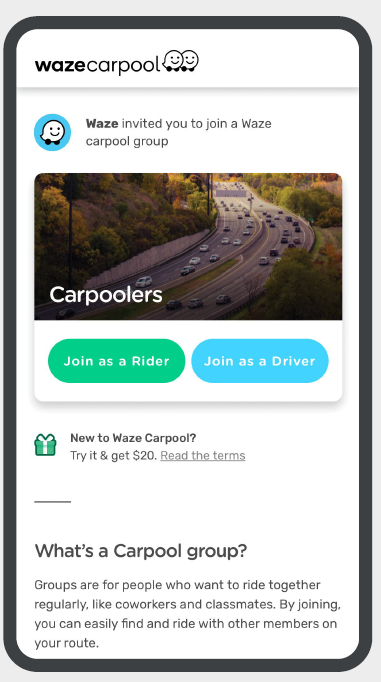
\includegraphics[width=0.25\textwidth]{./04-figuras/waze/Tela_de_grupos.png}
	\label{fig:tela_grupos_wazecarpool}
	\fonte{Programa de Parceria Brasil - Waze Carpool}
\end{figure}

A Waze oferece o serviço do aplicativo para diversas empresas que desejam incorporar a cultura das caronas entre seus empregados porque a empresa acredita que as caronas costumam aproximar mais as pessoas e criar momentos que no local de trabalho não existiriam.

O aplicativo tem uma dinâmica interessante, funciona a partir da criação de grupos, e os usuários destes grupos oferecem caronas entre si. Alunos de universidades como a UFRJ que por um tempo teve o seu próprio aplicativo de carona, o Caronaê, utilizam a ferramenta para pegar e oferecer a carona aos integrantes dos grupos que são criados e gerenciados por uma pessoa que ficar responsável pela comunicação da instituição com a empresa, o chamado "Embaixador".
% texto do material da waze 




\section{Veículos Compartilhados}
Na categoria de veículos compartilhados, separamos dois exemplos dos mais conhecidos com diferentes características cada. Há soluções desde compartilhamentos de bicicletas e automóveis.  %texto escrito por mim

Chips e cartões inteligentes ("\textit{smart-card}") são tecnologias bastante utilizadas nesse tipo de modelo de solução de mobilidade. Os chips utilizados em muitos casos para monitorar as bicicletas compartilhadas, e em algumas cidades, como Rennes na França, em 1998, utilizava os cartões inteligentes para a liberação das bicicletas nas estações.%mestrado da luisa

Aliás, Paris foi uma das primeiras cidades a utilizar os chamados sistemas de terceira geração, no qual a tecnologia utilizada é capaz de controlar o uso dos veículos em tempo real, GPS, cartões inteligentes, chips, todos, entram na lista dos dispositivos que possibilitam esse controle.

\subsection{Yellow}

Utilizando chips em seus veículos e QR Code para desbloquear seus veículos, a Yellow é uma startup brasileira de micromibilidade -- termo dado para veículos que servem para percorrer distâncias curtas -- que aluga bicicletas e partinetes elétricos fundada em 2017. Funcionando através de um serviço \textit{dockless}, ou seja, ao invés das bicicletas terem um ponto de estacionamento especifico, elas podem ser encontradas e deixadas em qualquer lugar que esteja dentro das áreas de atuação exibidas pelo aplicativo, podendo ser monitorada e controlada. 

Após o fim do uso, basta o usuário travar o cadeado que fica na bicicleta, que está pronta para o próximo usuário. A Yellow também utiliza o GPS, tanto para mostrar o trajeto percorrido pelo usuário quanto para apresentar onde estão as bicicletas no mapa. Na figura \ref{fig:yellow-app} é mostrado as áreas de atuação e a localização das bicicletas na cidade de São Paulo.

\begin{comment}
https://tecnoblog.net/286176/como-funciona-o-aluguel-de-bicicletas-e-patinetes-da-yellow/
\end{comment}

\begin{figure}[!hbtp]
	\centering
	\caption{Mapa do aplicativo Yellow na cidade de São Paulo}
	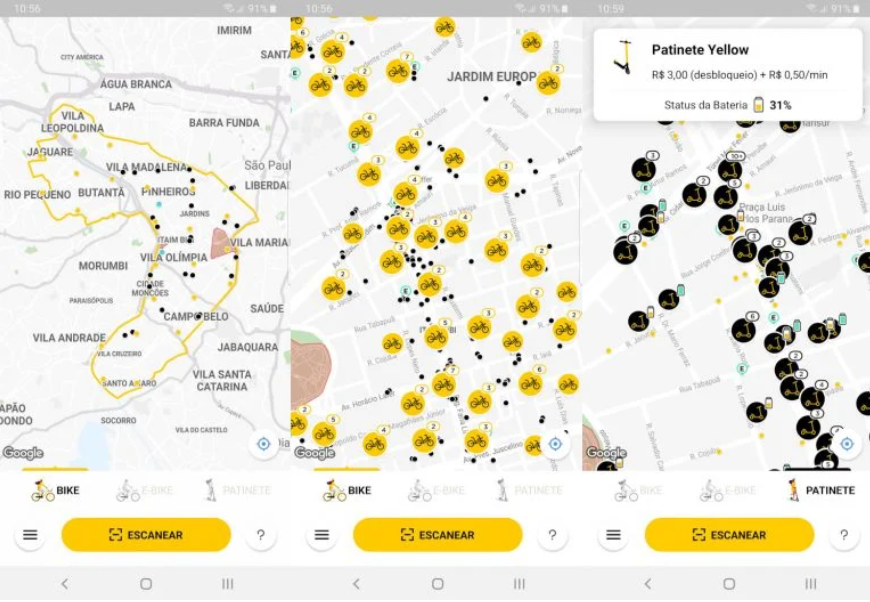
\includegraphics[width=0.6\textwidth]{./04-figuras/yellow/yellow.png}
	\label{fig:yellow-app}
	\fonte{https://tecnoblog.net/286176/como-funciona-o-aluguel-de-bicicletas-e-patinetes-da-yellow/} 
\end{figure}

\subsection{ZipCar}

Utilizando conceitos de \textit{Carsharing}, a empresa norte-americana que ainda não chegou com seus serviços no Brasil utiliza dos seus recursos tecnológicos -- aplicativo para dispositovos móveis -- para compartilhar carros entre seus usuários no estilo B2C (Business-to-Consumer). Semelhante a empresa Yellow, os usuários geralmente conseguem encontrar veículos próximos através de seus dispositivos móveis.

Segundo \cite{ballus-armet} os usuários do Zipcar precisam ao final do uso do veículo, devolvê-lo ao ponto de origem, algo que e chama de \textit{round-trip} ou ida e volta, modelo usado pela Zipcar. Outra empresa semelhante ao Zipcar é a Car2Go, divergindo no modelo de utilizaçao, na Car2Go o usuário deixa o veículo em uma localidade diferente por ser corridas chamadas \textit{one way}, ou seja, trecho único.

Ambos modelos de negócio estão relacionados a economia colaborativa e utilizam a plataforma da Internet, redes sociais, sistemas de informação e recursos tecnológico para oferecer o serviço e conectar seus usuários \cite{ballus-armet}. O aluguel são para pessoas que geralmente precisam de carros por poucas horas, % https://medium.com/@edselferri/o-case-zipcar-a7cbded4ba02#:~:text=Eles%20t%C3%AAm%20uma%20tecnologia%20sem,a%20torna%20um%20neg%C3%B3cio%20%C3%BAnico.
os clientes podem reservar um carro on-line e usar um cartão RFID chamado zipcard para entrar no carro reservado, passando o cartão no leitor perto do pára-brisa do motorista \cite{pearlson2009strategic} %\mnote{é um livro, precisa encontrar a página}.

%https://medium.com/@edselferri/o-case-zipcar-a7cbded4ba02#:~:text=Eles%20t%C3%AAm%20uma%20tecnologia%20sem,a%20torna%20um%20neg%C3%B3cio%20%C3%BAnico.
% texto copiado do site
Além de ter um serviço exclusivo, a Zipcar emprega tecnologia poderosa para dar suporte ao seu modelo de negócios \cite{pearlson2009strategic}. Eles têm uma tecnologia sem fio patenteada que é usada para monitorar a segurança do carro, o nível de feules, o uso por hora e outros recursos \cite{pearlson2009strategic}. A Zipcar desenvolveu um modelo de negócio único e apoiou-a com tecnologia apropriada, o que a torna um negócio único. Na figura \ref{fig:zipcar} mostra um usuário desbloqueando as portas do veículo da Zipcar.

\begin{figure}[!hbtp]
	\centering
	\caption{Como desbloquear seu Zipcar}
	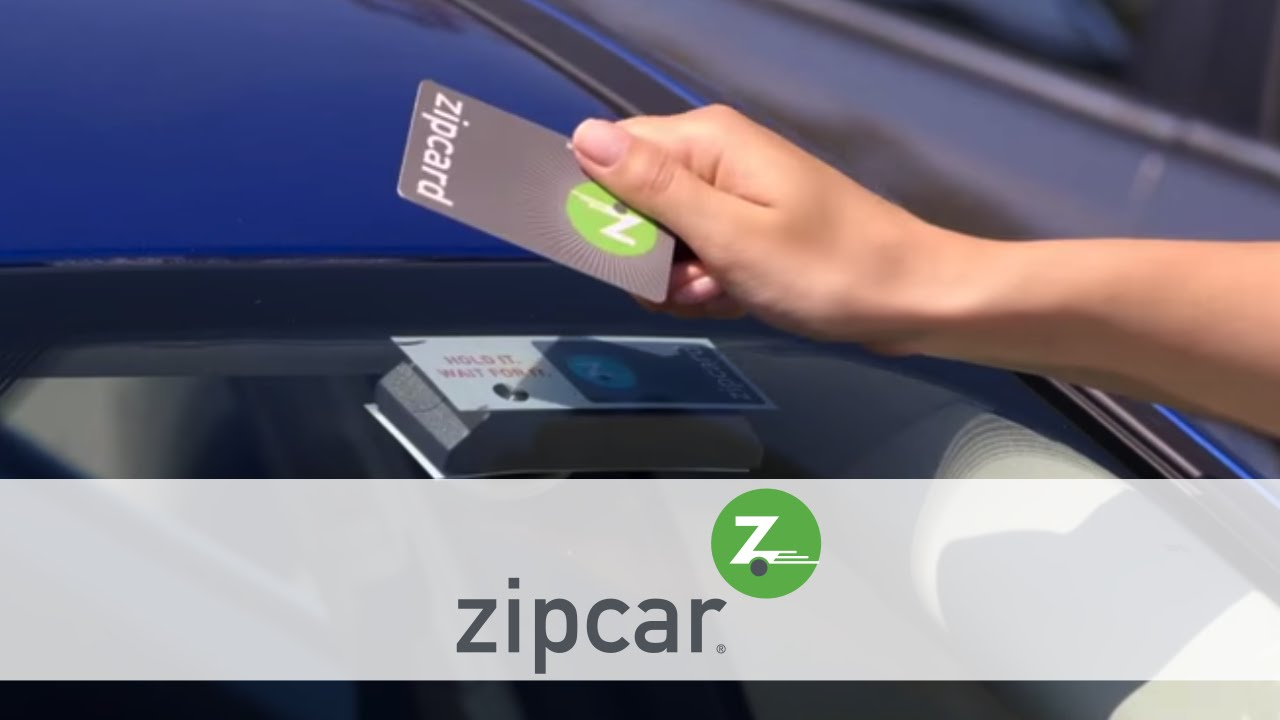
\includegraphics[width=0.8\textwidth]{./04-figuras/zipcar/zipcar.jpg}
	\label{fig:zipcar}
	\fonte{https://money.usnews.com/money/business-economy/articles/2008/06/05/5-keys-to-zipcars-success} %acesso: 13/04/2021 
\end{figure}



\begin{comment}
\section{Quadro Comparativo entre as soluções}
Depois de mostrar algumas das soluções existentes de mobilidade inteligente ao redor do mundo, vamos realizar uma comparação de qual solução será mais viável de ser implementada na Unifap levando em consideração o contexto local, as dificuldades de implementação e o questionário respondido pelo corpo docente e discente do Campus Macapá.

Levando em consideração o questionário que foi aplicado,logo de inicio, descartamos soluções de mobilidade inteligente que tem fins lucrativos e comerciais, como "Transporte Individual Privativo de Passageiros", além de não oferecerem nenhum serviço para o objetivo aqui proposto. Também, as "Orientações de Mobilidade" foram mencionadas para explanar sobre o tipo de mobilidade inteligente, porém, foge da ideia do projeto, pois não conseguiríamos oferecer o mínimo de garantia de segurança, praticidade e conforto.

As demais categorias mencionadas, "Viagens Compartilhadas" e "Veículos Compartilhados" foram analisados, e concluímos que seriam as mais viáveis. Excluímos as soluções privadas, que não garantiriam alguns requisitos mencionados no formulário, e analisamos 3 opções para oferecer, bicicletas compartilhadas, da categoria de veículos compartilhados e 2 soluções da categoria compartilhamento de corridas, Waze Carpool e Caronaê.

Os critérios foram baseados em cima das complexidade e contratempos que poderiam ter durante o processo de implementação, consideramos a infraestrutura institucional (UNIFAP) e da cidade de Macapá. Levamos em consideração também o custo tanto pro usuário, quanto pra universidade em organizar, gerenciar e manter os serviços da solução, além de necessidade futura de estar preparada para oferecer o serviço com qualidade independente do volume de dados. Soluções que já dispõem sua própria infraestrutura tecnológica parece atraente, porém, a maioria não fica dentro dos requisitos da comunidade da Unifap.

No quadro \ref{tab:quadro-solusdemobilidade} resume as características e modelos de negócios citados, apresentando algumas funcionalidades e regra de negócio de cada solução, além de expor quais soluções estão disponíveis para uso conforme as necessidades locais. O aplicativo Caronaê aparece como opção por ser de código aberto, e disponibiliza pelo GitHub a plataforma mobile, sua área administrativa e demais serviços, já o Waze Carpool nos da a possibilidade de criar grupos fechados, nos da todo o aparato tecnologico e as aplicações, nos dando apenas a responsabilidade de gerenciar os usuários e grupos. 


\begin{landscape}
	\begin{quadro}[]
		\caption{Soluções de mobilidade}
		\label{tab:quadro-solusdemobilidade}
		\resizebox{1.5\textwidth}{!}{%
			\begin{tabular}{|l|l|l|l|l|l|l|l|l|l|l|l|}
				\hline
				\multicolumn{12}{|c|}{Soluções de mobilidade} \\ \hline
				\multicolumn{1}{|c|}{Nome} &
				Categoria &
				\multicolumn{1}{c|}{\begin{tabular}[c]{@{}c@{}}Oferecer/Solicitar\\ Caronas\end{tabular}} &
				\multicolumn{1}{c|}{Proprietário} &
				\multicolumn{1}{c|}{\begin{tabular}[c]{@{}c@{}}Ambiente\\ administrativo \\ disponível a terceiros\end{tabular}} &
				\multicolumn{1}{c|}{Autenticação} &
				\multicolumn{1}{c|}{GPS} &
				\multicolumn{1}{c|}{\begin{tabular}[c]{@{}c@{}}Utiliza remuneração\\ no aplicativo\end{tabular}} &
				Plataforma &
				\begin{tabular}[c]{@{}l@{}}Identificação do \\ usuário\end{tabular} &
				Código aberto &
				Infraestrutura \\ \hline
				Waze &
				\begin{tabular}[c]{@{}l@{}}Orientação \\ de mobilidade\end{tabular} &
				Não &
				Waze Mobile &
				Não &
				\begin{tabular}[c]{@{}l@{}}Qualquer pessoa \\ que realizar o cadastro\end{tabular} &
				{\color[HTML]{000000} Sim} &
				Não &
				Android IOS &
				Conta cadastrada &
				Não &
				Própria \\ \hline
				Cittamobi &
				\begin{tabular}[c]{@{}l@{}}Orientação \\ de mobilidade\end{tabular} &
				Não &
				Cittati &
				Não &
				\begin{tabular}[c]{@{}l@{}}Qualquer pessoa \\ que realizar o cadastro\end{tabular} &
				Sim &
				Não &
				Android IOS &
				Conta cadastrada &
				Não &
				Própria \\ \hline
				Moovit &
				\begin{tabular}[c]{@{}l@{}}Orientação \\ de mobilidade\end{tabular} &
				Não &
				Moovit Inc. &
				Não &
				\begin{tabular}[c]{@{}l@{}}Qualquer pessoa \\ que realizar o cadastro\end{tabular} &
				Sim &
				Não &
				Android IOS &
				Conta cadastrada &
				Não &
				Própria \\ \hline
				Google Maps &
				\begin{tabular}[c]{@{}l@{}}Orientação \\ de mobilidade\end{tabular} &
				Não &
				Google &
				Não &
				\begin{tabular}[c]{@{}l@{}}Qualquer pessoa \\ que realizar o cadastro\end{tabular} &
				Sim &
				Não &
				Android IOS &
				Conta cadastrada &
				Não &
				Própria \\ \hline
				Uber &
				\begin{tabular}[c]{@{}l@{}}Transporte índividual\\ privado de passageiros\end{tabular} &
				Não &
				Uber Technologies Inc. &
				Não &
				\begin{tabular}[c]{@{}l@{}}Qualquer pessoa \\ que realizar o cadastro\end{tabular} &
				Sim &
				Sim &
				Android IOS &
				Conta cadastrada &
				Não &
				Própria \\ \hline
				99 &
				\begin{tabular}[c]{@{}l@{}}Transporte índividual\\ privado de passageiros\end{tabular} &
				Não &
				Didi Chuxing &
				Não &
				\begin{tabular}[c]{@{}l@{}}Qualquer pessoa \\ que realizar o cadastro\end{tabular} &
				Sim &
				Sim &
				Android IOS &
				Conta cadastrada &
				Não &
				Própria \\ \hline
				Blablacar &
				Viagens compartilhadas &
				Sim &
				Comuto SA &
				Não &
				\begin{tabular}[c]{@{}l@{}}Qualquer pessoa \\ que realizar o cadastro\end{tabular} &
				Não &
				Sim &
				Android IOS &
				Conta cadastrada &
				Não &
				Própria \\ \hline
				Yellow &
				Veículos compartilhados &
				Não &
				Grow &
				Não &
				\begin{tabular}[c]{@{}l@{}}Qualquer pessoa \\ que realizar o cadastro\end{tabular} &
				Sim &
				Sim &
				Android IOS &
				Conta cadastrada &
				Não &
				Própria \\ \hline
				Cabify &
				Viagens compartilhadas &
				Não &
				Juan de Antonio &
				Não &
				\begin{tabular}[c]{@{}l@{}}Qualquer pessoa \\ que realizar o cadastro\end{tabular} &
				Sim &
				Sim &
				Android IOS &
				Conta cadastrada &
				Não &
				Própria \\ \hline
				Bynd &
				Viagens compartilhadas &
				Não &
				&
				Não &
				\begin{tabular}[c]{@{}l@{}}Qualquer pessoa \\ que realizar o cadastro\end{tabular} &
				Sim &
				Sim &
				Android IOS &
				Conta cadastrada &
				Não &
				Própria \\ \hline
				Vemcar &
				Viagens compartilhadas &
				Sim &
				UFMG &
				Não &
				\begin{tabular}[c]{@{}l@{}}Somente alunos da \\ UFMG\end{tabular} &
				Sim &
				Recompensas &
				Android &
				\begin{tabular}[c]{@{}l@{}}Sistema de Gestão\\ da UFMG\end{tabular} &
				Não &
				UFMG \\ \hline
				ZipCar &
				Veículos compartilhados &
				Não &
				Avis Budget Group &
				Não &
				\begin{tabular}[c]{@{}l@{}}Qualquer pessoa \\ que realizar o cadastro\end{tabular} &
				Sim &
				Sim &
				Android IOS &
				Conta cadastrada &
				Não &
				Própria \\ \hline
				Caronaê &
				Viagens compartilhadas &
				Sim &
				UFRJ &
				Sim &
				\begin{tabular}[c]{@{}l@{}}Somente alunos da \\ UFRJ\end{tabular} &
				Não &
				Não &
				Android IOS &
				\begin{tabular}[c]{@{}l@{}}Sistema de Gestão \\ da UFRJ\end{tabular} &
				%\cellcolor[HTML]{FFFC9E}
				Sim &
				UFRJ \\ \hline
				Waze Carpool &
				Viagens compartilhadas &
				Sim &
				Waze Mobile &
				%\cellcolor[HTML]{FCFF2F}
				Sim &
				\begin{tabular}[c]{@{}l@{}}Qualquer pessoa \\ que realizar o cadastro\end{tabular} &
				Sim &
				Sim &
				Android IOS &
				Conta cadastrada &
				Não &
				Própria \\ \hline
			\end{tabular}%
		}
	\end{quadro}
\end{landscape}
\end{comment}